\documentclass{beamer}

\usepackage{helvet}
\usepackage{hyperref, graphicx}
\usepackage{amsthm}
\usepackage{etoolbox}
%\usepackage{multicol}
\usepackage{tikz}
\usepackage{ulem}

\usetheme{default}
\setbeamertemplate{navigation symbols}{}
\AtBeginSection[ ]
{
\begin{frame}{Outline}
    \tableofcontents[currentsection]
\end{frame}
}

% Default fixed font does not support bold face
\DeclareFixedFont{\ttb}{T1}{txtt}{bx}{n}{11} % for bold
\DeclareFixedFont{\ttm}{T1}{txtt}{m}{n}{12}  % for normal - use in headings

% Custom colors
\usepackage{color}
\definecolor{TUGray}{RGB}{101,101,137}
\definecolor{TUBlack}{RGB}{30,0,0}
\definecolor{mygreen}{RGB}{45,111,63}
\definecolor{keywords}{RGB}{205,114,0}
\definecolor{comments}{RGB}{181,51,139}
\definecolor{strings}{RGB}{58,144,81}
\definecolor{numeric}{RGB}{66,110,176}
\definecolor{linos}{rgb}{0.4,0.4,0.4}
\definecolor{links}{rgb}{0,0.4,0.75}

\definecolor{bggray}{RGB}{232, 233, 235}

\usecolortheme[named=mygreen]{structure}
\setbeamercolor{normal text}{fg=TUBlack}\usebeamercolor*{normal text}

\setbeamercolor{codecol}{fg=TUGray!25!black,bg=bggray}

\hypersetup{colorlinks, linkcolor=links, urlcolor=links}

\usepackage[T1]{fontenc}
\usepackage[sfdefault,scaled=.85]{FiraSans}
\usepackage{newtxsf}

\usepackage{listings}

\newtoggle{InString}{}% Keep track of if we are within a string
\togglefalse{InString}% Assume not initally in string

\newcommand\digitstyle{\color{numeric}}
\makeatletter
\newcommand{\ProcessDigit}[1]
{%
  \ifnum\lst@mode=\lst@Pmode\relax%
   {\digitstyle #1}%
  \else
    #1%
  \fi
}
\makeatother

\lstset{literate=%
    {0}{{{\ProcessDigit{0}}}}1
    {1}{{{\ProcessDigit{1}}}}1
    {2}{{{\ProcessDigit{2}}}}1
    {3}{{{\ProcessDigit{3}}}}1
    {4}{{{\ProcessDigit{4}}}}1
    {5}{{{\ProcessDigit{5}}}}1
    {6}{{{\ProcessDigit{6}}}}1
    {7}{{{\ProcessDigit{7}}}}1
    {8}{{{\ProcessDigit{8}}}}1
    {9}{{{\ProcessDigit{9}}}}1
	{<=}{{\(\leq\)}}1
	{>=}{{\(\geq\)}}1,
	% morestring=[b]",
    % morestring=[b]',
    % morecomment=[l]{//},
}

\lstdefinelanguage{Pseudo}{
    morekeywords={return, while, if, for, input},
    morecomment=[l]{\#},
}

% Pseudocode style
\newcommand\pseudostyle{\lstset{
language=Pseudo,
basicstyle=\fontfamily{ccr}\scriptsize,
commentstyle=\it\scriptsize\color{linos},
keywordstyle=\it\bfseries\scriptsize,
mathescape=true,
literate=
    {=}{$\leftarrow{}$}{1}
    {==}{$={}$}{1}
    {<=}{{\(\leq\)}}1
	{>=}{{\(\geq\)}}1,
xleftmargin=18pt,
xrightmargin=4pt,
aboveskip=12pt,
belowskip=0pt,
frame=tB,
keepspaces=true
}}

% Python style for highlighting
\newcommand\pythonstyle{\lstset{
language=Python,
basicstyle=\ttfamily\tiny,
numbers=left,
numberstyle=\tiny\color{linos},
morekeywords={self, np},              % Add keywords here
keywordstyle=\tiny\color{keywords},
commentstyle=\it\tiny\color{comments},    % Custom highlighting style
stringstyle=\tiny\color{strings},
xleftmargin=18pt,
xrightmargin=4pt,
aboveskip=0pt,
belowskip=0pt,
escapeinside={(*@}{@*)},
frame=l,                         % Any extra options here
showstringspaces=false,
keepspaces=true
}}

% Pseudocode environment
\lstnewenvironment{pseudo}[1][]
{
    \pseudostyle
    \lstset{
        #1
    }
}
{}

% Python environment 
\lstnewenvironment{python}[1][]
{
	\pythonstyle
	\lstset{
	#1
	}
}
{}

% wrap the Python environment
\newenvironment{codeblock}
    {\hfill\begin{beamerboxesrounded}[lower=codecol, width=0.8\textwidth]
    \medskip

    }
    { 
    \end{beamerboxesrounded}\hfill
    }

\theoremstyle{example}
\newtheorem{question}{Question}

\newcommand{\ct}[1]{\lstinline[language=Python]!#1!}
\newcommand{\ttt}[1]{{\small\texttt{#1}}}
\newcommand{\lsitem}[2]{\ttt{{#1}[}\ct{#2}\ttt{]}}

\author{Chris Cornwell}
\date{Mar 13, 2025}
\title{Overview of Machine Learning \newline 
    \footnotesize{in particular, Supervised Learning}}

\begin{document}

\begin{frame}
\titlepage
\end{frame}

\begin{frame}
\frametitle{Outline}
\tableofcontents
\end{frame}

\section{Machine Learning}

%%%%
\begin{frame}
\frametitle{What is Machine Learning?}
    % Mitchell '98 ``Well posed learning problem''
    Definition by Tom Mitchell:\newline 
    \begin{quote}
        A ``computer program'' is said to \textbf{learn} from experience $E$, with respect to some task $T$ and performance measure $P$ if: its performance on $T$, as measured by $P$, improves with experience $E$.
    \end{quote}
    \begin{itemize}
        \item The definition is intentionally general. Often, could think of $E$ as ``training'' (updates to how program runs), based on observed data.
        \item ``computer program'' (for us) means a procedure or function, implemented on a computer, that produces output from given input. The output is how the program is supposed to achieve the task $T$. 
        \item The procedures discussed in class {--} linear regression and the Perceptron algorithm for half-space model {--} fit into this paradigm\ldots \textit{kind of}.
    \end{itemize}

\end{frame}

%%%%
\begin{frame}
\frametitle{What is Machine Learning?}
    Definition by Tom Mitchell:\newline 
    \begin{quote}
        A computer program is said to \textbf{learn} from experience $E$, with respect to some task $T$ and performance measure $P$ if: its performance on $T$, as measured by $P$, improves with experience $E$.
    \end{quote}
    
    {\color{mygreen}Examples:}
    \begin{enumerate}
        \item Linear regression.
        \begin{itemize}
            \item ``program'': the process taking input ($x$, potentially multiple variables), ``predicting'' a label $\hat{y}$. (with $\hat{y} = \hat{m}x + \hat{b}$.)
            \item $T$: fit observed points $(x_1,y_1),\ldots,(x_n,y_n)$ well with predictions $(x_1,\hat{y}_1), \ldots,(x_n,\hat{y}_n)$, with expectation of good fit on \textit{unobserved} data.
            \item $E$: ?? \newline 
                    The data are used to get $\hat{m}$ and $\hat{b}$, but you don't really ``improve'' with repeated use of data. \newline 
                    A \emph{closed form} for best choice of $\hat{m}, \hat{b}$: compute $(A^TA)^{-1}A^T{\bf y}$.
            \item $P$: Mean squared error.
        \end{itemize}
        One should not expect nice closed form in general.
    \end{enumerate}

\end{frame}

%%%%
\begin{frame}
\frametitle{What is Machine Learning?}
    Definition by Tom Mitchell:\newline 
    \begin{quote}
        A computer program is said to \textbf{learn} from experience $E$, with respect to some task $T$ and performance measure $P$ if: its performance on $T$, as measured by $P$, improves with experience $E$.
    \end{quote}
    
    {\color{mygreen}Examples:}
    \begin{enumerate}
        \setcounter{enumi}{1}
        \item The Perceptron algorithm.
        \begin{itemize}
            \item ``program'': the process taking input (${\bf x}\in \mathbb R^d$, or something \textit{turned into} ${\bf x}\in\mathbb R^d$), ``predicting'' a label $+1$ or $-1$. (using $W = ({\bf w}, b)\in\mathbb R^{d+1}$ to decide label.)
            \item $T$: predicting labels correctly\ldots including on \textit{unobserved} data.
            \item $E$: looking through observed data $X_i = ({\bf x}_i,1)$, label $y_i$, and updating $W^{(t+1)} = W^{(t)} + y_iX_i$ when $i$ found with $W^{(t)}\cdot(y_iX_i)\le 0$.
            \item $P$: ?? \newline 
                    Whether its labels on all observed data are correct. But, only two results: \textit{True} or \textit{False}. \newline 
                    If data is linearly separable, enough of experience $E$ improves this measure (changing to \textit{True}). Only happens if linearly separable.
        \end{itemize}
    \end{enumerate}

\end{frame}

%%%%
\begin{frame}
\frametitle{What types of \emph{tasks} and \emph{algorithms} in machine learning?}
% Supervised learning 
    % examples
% Unsupervised learning 
    % examples
% Reinforcement learning
    %example
% some others
\end{frame}

\section{Supervised learning}

%%%%
\begin{frame}
\frametitle{The goal of supervised learning}
% an ``input space'' $\mathbb R^{d}$ (could be more general space) and output space, or label space, $Y$; it may be that $Y\subseteq \mathbb R^m$ for some $m$ -- change it to this?.
% get a sample $\mathcal S = \{({\bf x}_i, y_i)\}_{i=1}^n$ that is drawn from an (unknown) probability distribution on $\mathbb R^{d}\times Y$, $P_{X,Y}:\mathbb R^{d}\times Y \to [0, \infty)$ 
% goal: learn from $\mathcal S$ a function that predicts $y$ from ${\bf x}\in\mathbb R^d$ (well) 

\end{frame}

%%%%
\begin{frame}
\frametitle{How to achieve the goal}
    % choose a parameterized function class; your predictor function will come from that class

\end{frame}

%%%%
\begin{frame}
    \frametitle{Linearly separable}
    \begin{figure}[h!]
        \centering
        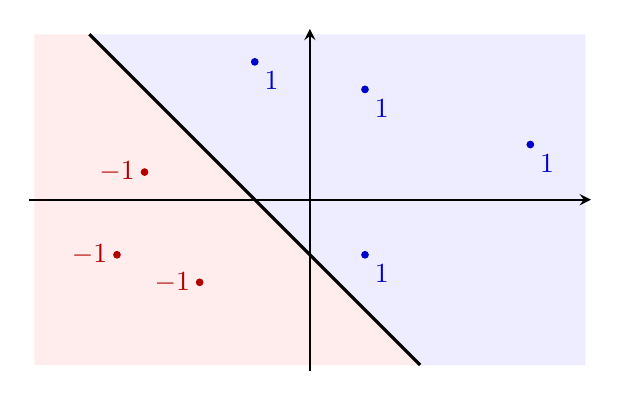
\begin{tikzpicture}[>=stealth, scale=0.7]
            \fill[blue!35!white, opacity = 0.2] (-4, 3) -- (5, 3) -- (5, -3) -- (2, -3)-- cycle;
            \fill[red!35!white, opacity = 0.2] (-4, 3) -- (-5, 3) -- (-5, -3) -- (2, -3)-- cycle;
            \draw[thick, ->] (-5.1, 0)-- (5.1, 0); 
            \draw[thick, ->] (0, -3.1) -- (0, 3.1); 
            \draw[very thick] (-4, 3) -- (2, -3); % node[above right]{\small $H = \{x + y + 1 = 0\}$}; 
            \fill[blue!80!black] (1, 2)node[below right]{$1$} circle (2pt); 
            \fill[blue!80!black] (-1, 2.5)node[below right]{$1$} circle (2pt); 
            \fill[blue!80!black] (1, -1)node[below right]{$1$} circle (2pt); 
            \fill[blue!80!black] (4, 1)node[below right]{$1$} circle (2pt); 
            \fill[red!70!black] (-3, 0.5)node[left]{$-1$} circle (2pt); 
            \fill[red!70!black] (-3.5, -1)node[left]{$-1$} circle (2pt); 
            \fill[red!70!black] (-2, -1.5)node[left]{$-1$} circle (2pt); 
        \end{tikzpicture}
        \caption{The hyperplane $H = \{(x_1,x_2)\in \mathbb R^2: x_1+ x_2+ 1 = 0\}$, corresponding positive and negative regions, ${\bf w} = (1, 1)$, $b = 1$}
        \label{figure:R2HyperplaneLabeled}
    \end{figure}
\end{frame}

%%%%
\begin{frame}
    \frametitle{Not linearly separable}
    \begin{figure}[h!]
        \centering
        \begin{tikzpicture}[>=stealth, scale=0.7]
            %\fill[blue!35!white, opacity = 0.2] (-4, 3) -- (5, 3) -- (5, -3) -- (2, -3)-- cycle;
            %\fill[red!35!white, opacity = 0.2] (-4, 3) -- (-5, 3) -- (-5, -3) -- (2, -3)-- cycle;
            \draw[thick, ->] (-5.1, 0)-- (5.1, 0); 
            \draw[thick, ->] (0, -3.1) -- (0, 3.1); 
            %\draw[very thick] (-4, 3) -- (2, -3); % node[above right]{\small $H = \{x + y + 1 = 0\}$}; 
            \fill[blue!80!black] (1, 2)node[below right]{$1$} circle (2pt); 
            \fill[red!70!black] (1, -1)node[below right]{$-1$} circle (2pt); 
            \fill[red!70!black] (-3, 0.5)node[left]{$-1$} circle (2pt); 
            \fill[blue!80!black] (-2, -1.5)node[left]{$1$} circle (2pt); 
        \end{tikzpicture}
        \caption{A data set in $\mathbb R^2$ that is not linearly separable.}
        \label{figure:notseparable}
    \end{figure}
    \pause
    \begin{itemize}
        \item A criterion (checkable, in theory) that is equivalent to ``not linearly separable''?
    \end{itemize}
\end{frame}

\section{Perceptron algorithm}

%%%%
\begin{frame}
    \frametitle{Setup for Perceptron algorithm}
    Labeled data: $({\bf x}_1, y_1), \ldots, ({\bf x}_n, y_n)$, with ${\bf x}_i\in\mathbb R^d$ and $y_i\in\{\pm1\}$ for all $i$.

    Assuming labeled data is linearly separable, the Perceptron algorithm is a procedure that is guaranteed to find a hyperplane that separates the data.\footnote{Introduced in \textit{The perceptron: A probabilistic model for information storage and organization in the brain}, F.~Rosenblatt, Psychological Review \textbf{65} (1958), 386{--}407.}
    
    \pause
    To describe it: for each ${\bf x}_i$, use $X_i$ to denote the $(d+1)$-vector consisting of ${\bf x}_i$ with $1$ appended at the end;

    Additionally, use $W$ to denote the vector ${\bf w}$ with $b$ appended at the end.

    \pause
    Note that $W\cdot X_i = {\bf w}\cdot{\bf x}_i + b$. 

    For linearly separable data, our goal is to find $W\in\mathbb R^{d+1}$ so that $W\cdot X_i$ and $y_i$ have the same sign (both positive or both negative), for all $1\le i\le n$.
    \begin{itemize}
        \item Equivalently, we need $y_i W\cdot X_i > 0$ for all $1\le i\le n$.
    \end{itemize}
\end{frame}

%%%%
\begin{frame}[fragile]
\frametitle{Perceptron algorithm}
Suppose the data is linearly separable. Also, \ttt{x} is an $n\times d$ array of points, with i$^{th}$ row equal to ${\bf x}_i$, and \ttt{y} is array of the labels. The Perceptron algorithm finds \ttt{W} iteratively as follows.\footnote{Recall, in pseudo-code block, left-facing arrow means \textit{assign} to variable on left.}
\pause 

\begin{pseudo}
input: x, y  ## x is n by d, y is 1d array
X = append 1 to each row of x
W = (0,0,...,0)  ## Initial W
while (exists i with y[i]*dot(W, X[i]) <= 0){
    W = W + y[i]*X[i]
}
return W
\end{pseudo}

\end{frame}

%%%%
\begin{frame}
    \frametitle{Perceptron algorithm, stopping time}
    Under our assumptions for Perceptron algorithm, a guarantee on eventually stopping.

    \begin{theorem}Define $R = \max_i|X_i|$ and $B = \min_i\{|V|: \forall i, y_iV\cdot X_i \ge 1\}$. Then, the Perceptron algorithm stops after at most $(RB)^2$ iterations and, when it stops with output $W$, then $y_iW\cdot X_i > 0$ for all $1\le i\le n$.
    \end{theorem}

    \pause 
    \textbf{Idea of proof:} Write $W^*$ for vector that realizes the minimum $B$. Also, write $W^{(t)}$ for the vector $W$ on the $t^{th}$ step, with $W^{(1)} = (0,0,\ldots,0)$.

    \pause
    Using how $W^{(t+1)}$ is obtained from $W^{(t)}$, can show that $W^*\cdot W^{(T+1)} \ge T$ after $T+1$ iterations. Also, using the condition on $W^{(T)}$ that necessitates an update, can show that $|W^{(T+1)}| \le \sqrt{T}R$. (Both statements, use induction.) 

    \pause
    Now, by Cauchy-Schwarz inequality, $T \le BR\sqrt{T}$, which we can rearrange to $T\le (BR)^2$.
\end{frame}
\end{document}